We present some examples that illustrates the use of Qlang in solving quantum computing problems.

\subsection { Solving Quantum Computation Problem}
\subsubsection{Problem1}
Evaluate the following expressions: a. $(H \otimes S) \ket{00}$ b. $\dotproduct[101,000]$ c. $\bra{01} H \otimes H \ket{01} $
\subsubsection{Problem 2}
Find the matrix corresponding to the quantum circuit:
\begin{figure}[h!]
\begin{center}
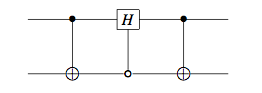
\includegraphics{circuit1}
\end{center}
\caption{ Quantum Circuit implementing series of control gates
\label{cir1}}
\end{figure}

\begin{lstlisting}
def circuitMat = findMatrix (){
	qubit mat0=|00>;
	qubit mat1=|01>;
	qubit mat2=|10>;
	qubit mat3=|11>;
		
		
	CNOT = [1,0,0,0;0,1,0,0;0,0,0,1;0,0,1,0]
	HNOT = [1/sqrt(2),0,0,1/sqrt(2);0,1,0,0;1/sqrt(2),0,1,-1/sqrt(2);0,0,0,0]
	allGates = CNOT * HNOT * CNOT
		
	circuitMat =[allGates*mat0:allGates*mat1:allGates*mat2:allGates*mat3]
		
	}
\end{lstlisting}
\subsubsection{Problem 3}
Consider the circuit and show the probabilities of outcome 0 and 1.
\begin{figure}[h!]
\begin{center}
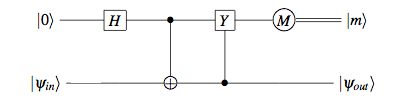
\includegraphics{circuit2}
\end{center}
\caption{ Quantum Circuit 
\label{cir1}}
\end{figure}

\subsection{Deutsch Jozsa Algorithm}
\begin{lstlisting}

	def outcome = deutschJozsa(qubit in, mat U){
		
		mat qubitInput;
		qubitInput = in @ |1>;
		input = (H @ H)*input;
		input = U * input;
		input = (H @ I)*input;
		input=(in*Adj(in)@ I)*input;
		
		if (input == 0){
			outcome = 0;
		}
		else{
			outcome = 1;
		}
	}
	
\end{lstlisting}
